\PassOptionsToPackage{table}{xcolor}
\documentclass[10pt]{beamer}
\usepackage[english]{babel}

\usetheme{metropolis}
\usepackage{smartdiagram}
\usepackage{listings}
\usepackage{booktabs}
\usepackage[scale=2]{ccicons}%creative commons
\setbeamercovered{transparent}%invisible by default
\usepackage{array}
\newcolumntype{L}[1]{>{\raggedright\let\newline\\\arraybackslash\hspace{0pt}}m{#1}}
\newcolumntype{C}[1]{>{\centering\let\newline\\\arraybackslash\hspace{0pt}}m{#1}}
\newcolumntype{R}[1]{>{\raggedleft\let\newline\\\arraybackslash\hspace{0pt}}m{#1}}

\usepackage{pgfplots}
\usepgfplotslibrary{dateplot}
\usepackage{tikz}
\usepackage{tikz-uml}
\usetikzlibrary{positioning,chains,fit,shapes,calc,automata,positioning}
\newcommand{\mycomment}[1]{}
\usepackage{fancyvrb}
\usepackage{ifpdf}                        % To check if pdflatex is used.

\ifpdf
  \DeclareGraphicsRule{*}{mps}{*}{}       % To include metapost files.
\fi
% *****************************************************************************
% Matematica 
% *****************************************************************************

%\usepackage{amssymb}
%\usepackage{mathtools}                    % Add support for cramped,
					  
%\usepackage[euler]{flexisym}
%\usepackage{breqn}                        % Breqn
%\makeatletter
%   \def\eqnumsize{\normalfont \Tf@font}      % Add support to Minion Pro
%\makeatother
%\setkeys{breqn}{labelprefix={eq:}}


%\usepackage{asymptote}
%\usepackage[loop, controls]{animate}

\graphicspath{{./}, {./Images/}}

\lstdefinelanguage{Kotlin}{
  keywords={package, as, typealias, this, super, val, var, fun, for, null, true, false, is, in, throw, return, break, continue, object, if, try, else, while, do, when, yield, typeof, yield, typeof, class, interface, enum, object, override, public, private, get, set, import, abstract, },
  keywordstyle=\color{blue}\bfseries,
  ndkeywords={@Deprecated, Int, Integer, Float, Double, String, Runnable, dynamic},
  ndkeywordstyle=\color{red}\bfseries,
  emph={println, return@, forEach,},
  emphstyle={\color{red}},
  identifierstyle=\color{black},
  sensitive=true,
  commentstyle=\color{gray}\ttfamily,
  comment=[l]{//},
  morecomment=[s]{/*}{*/},
  stringstyle=\color{gray}\ttfamily,
  morestring=[b]",
  morestring=[s]{"""*}{*"""},
}

\providecommand{\ie}{i.\,e.}
\providecommand{\Ie}{I.\,e.}
\providecommand{\eg}{e.\,g.}
\providecommand{\Eg}{E.\,g.} 

\metroset{block=fill}
\metroset{titleformat frame=smallcaps}

\title{Having fun with Kotlin coroutines}
%\subtitle{Ariadne's thread in Kotlin models of concurrency}
\subtitle{A first tour of concurrency models in Kotlin}

\date{\today}
\author[A. Candolini]{Alessandro Candolini}
%\institute{Department of Physics, University of Trieste}
% \titlegraphic{\hfill\includegraphics[height=1.5cm]{logo/logo}}

\begin{document}

\maketitle

\begin{frame}{Agenda}
  \setbeamertemplate{section in toc}[sections numbered]
  \tableofcontents[hideallsubsections]
\end{frame}

\section{We live in a concurrent world}
\begin{frame}[fragile]
	\begin{figure}
		\centering
		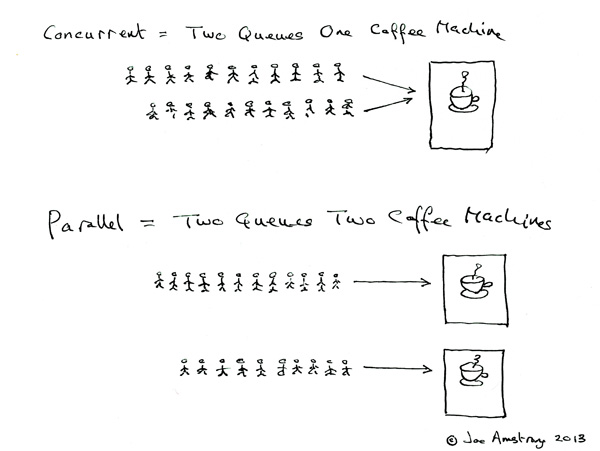
\includegraphics[width=.8\textwidth]{concurrency_coffee}
		\caption{\url{https://joearms.github.io/published/2013-04-05-concurrent-and-parallel-programming.html}}
	\end{figure}
\end{frame}
\begin{frame}[fragile]
Is concurrency relevant for mobile development?
	\begin{itemize} 
		\item<2-> IO (\eg, network, etc) 
		\item<3-> sensors (\eg, gps, etc) 
		\item<4-> UI events 
		\item<5-> platform lifecycle 
	\end{itemize}
\end{frame}
\begin{frame}[fragile]
\begin{columns}
\begin{column}{0.4\textwidth}
	\begin{center}
	\begin{figure}
		\centering
		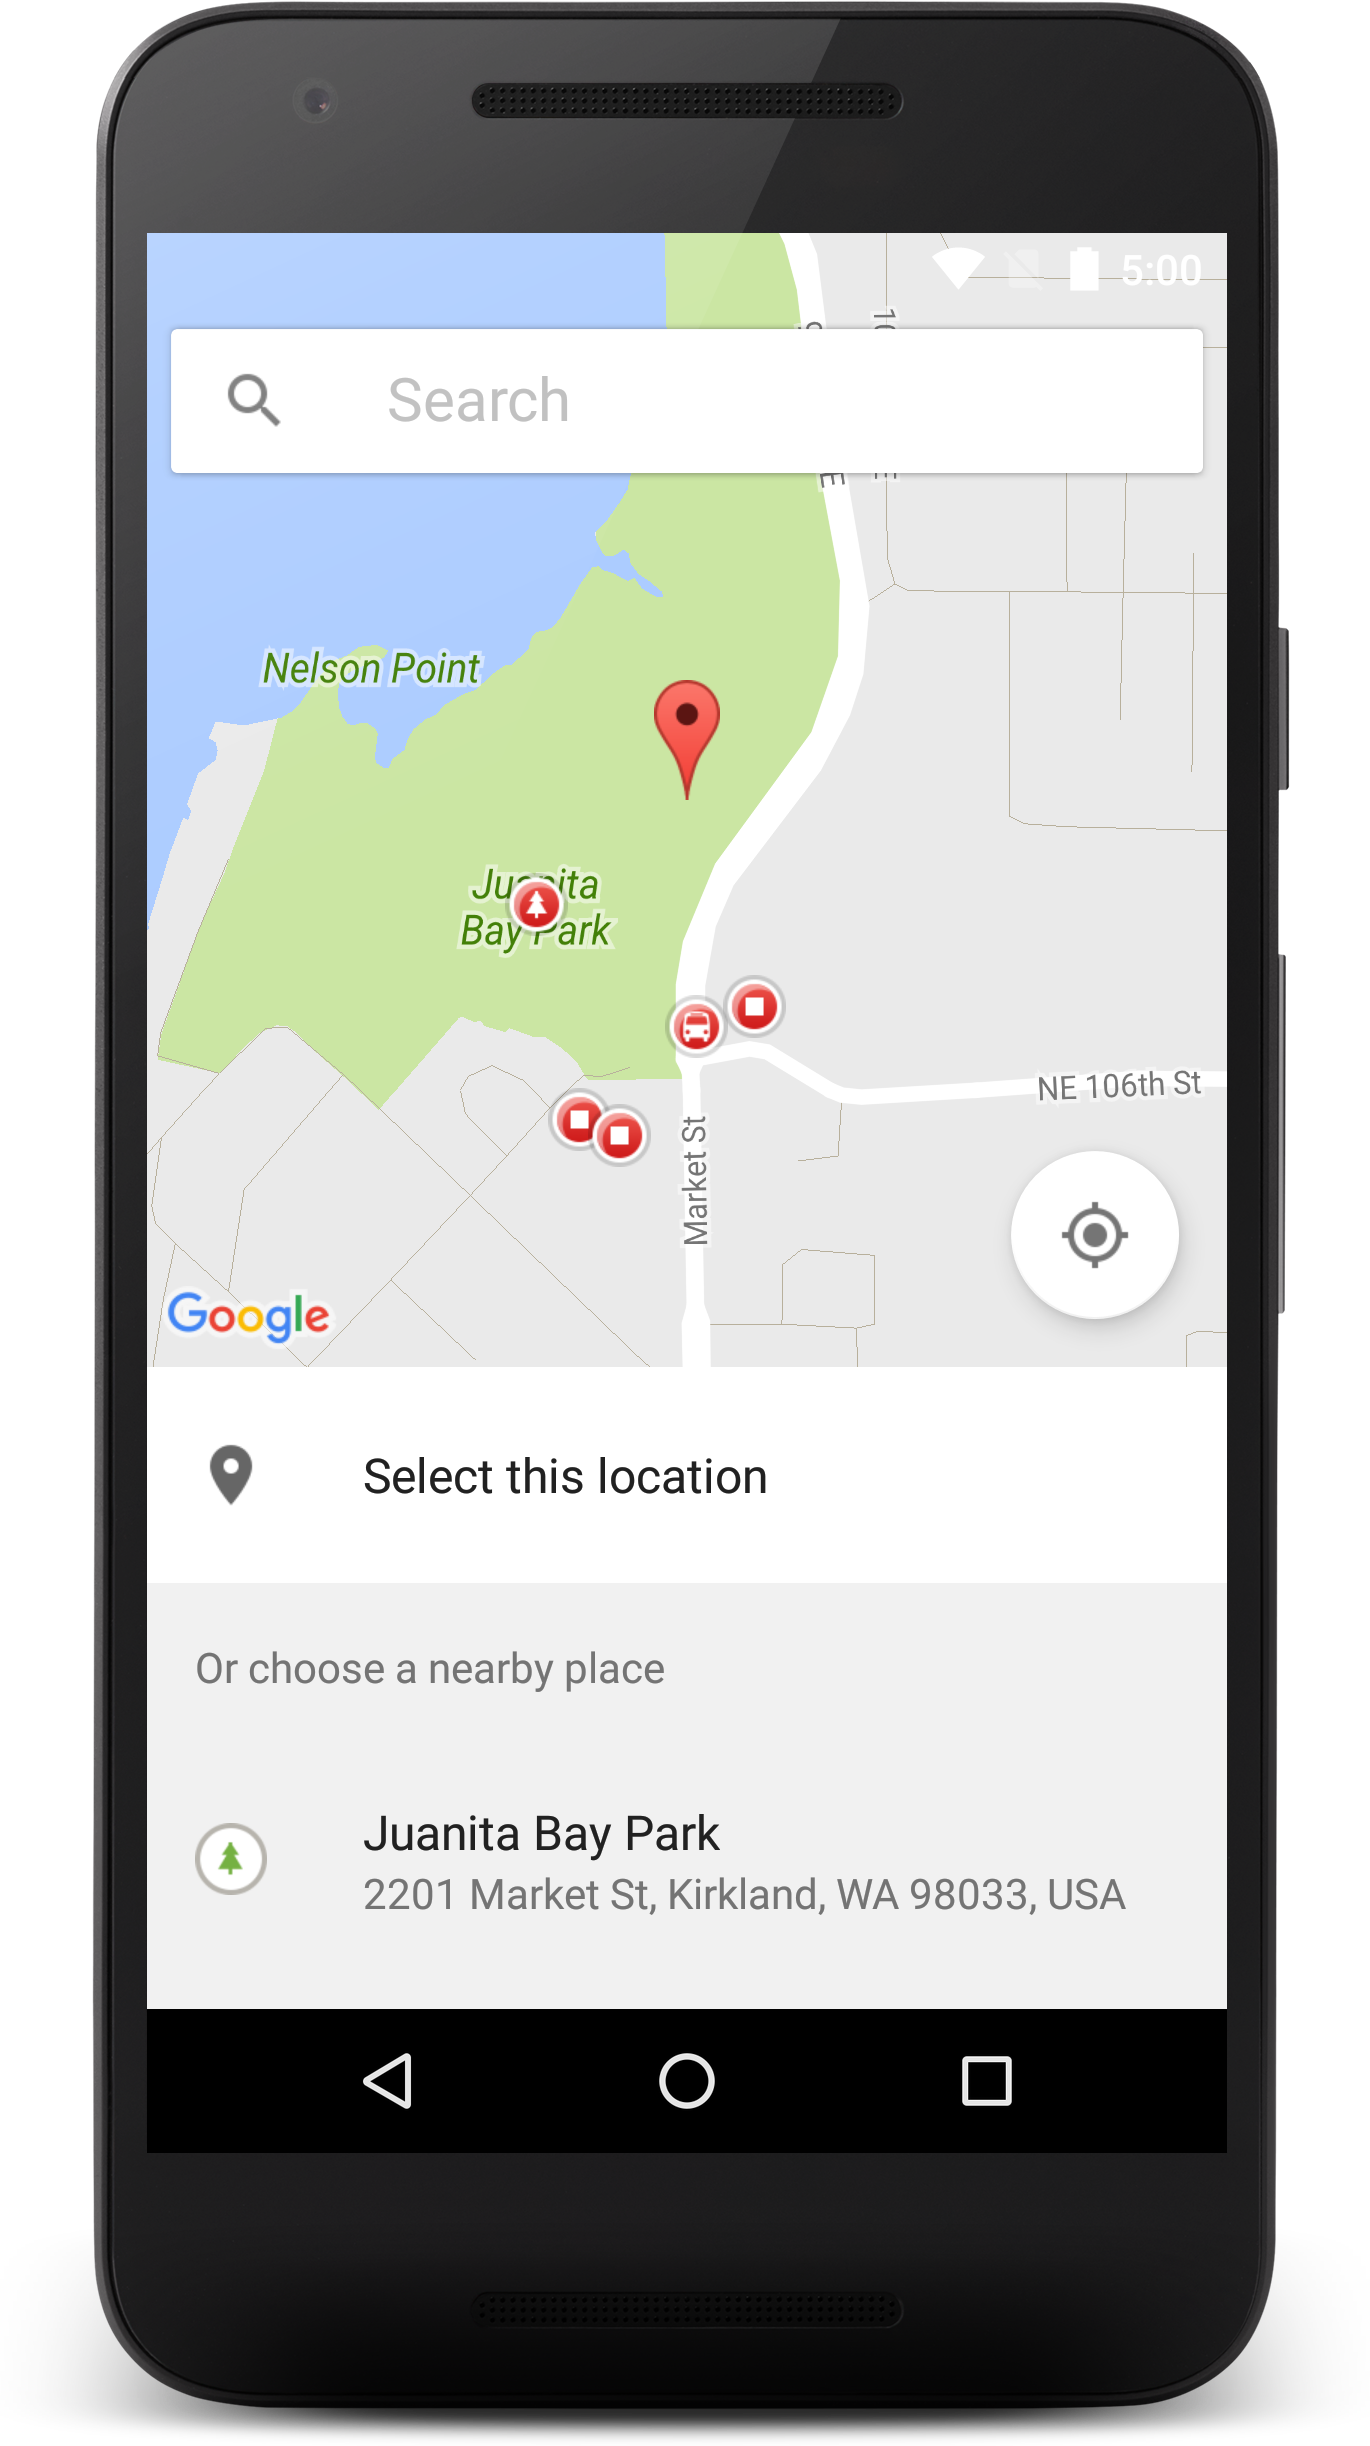
\includegraphics[height=.8\textheight]{location}
	\end{figure}
	\end{center}
\end{column}
\begin{column}{0.6\textwidth}
	acceptance criteria:
	\begin{itemize}
		\item search by current location 
		\item search by location name 
	\end{itemize}
	advanced 
	\begin{itemize}
		\item search suggestions when tying 
	\end{itemize}
\end{column}
\end{columns}
\end{frame}
\begin{frame}[fragile]
	Translate ACs into code: simple \emph{sequential} state machine  (simplified) 
	\begin{figure}
		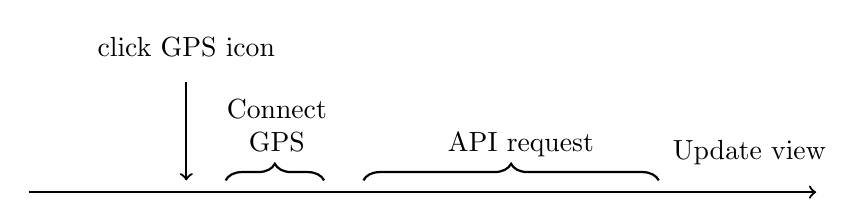
\begin{tikzpicture}[scale=1]
%\node[align=center] at (1,0.5) {Enter};
\node[align=center] at (2,1.85) {click GPS icon};
\draw [thick,->] (2,1.4) -- (2,0.15);
\node[align=center] at (3.15,0.85) {Connect\\GPS};
\draw [thick,decorate,decoration={brace,amplitude=6pt,raise=0pt}] (2.5,0.15) -- (3.75,0.15);
%\draw [thick,->] (4,0.85) -- (4,0.15);
\node[align=center] at (6.25,0.6) {API request};
%\draw [thick,->] (8.25,0.85) -- (8.25,0.15);
\node[align=center] at (9.15,0.5) {Update view};
\draw [thick,decorate,decoration={brace,amplitude=6pt,raise=0pt}] (4.25,0.15) -- (8,0.15);
\draw [thick,->] (0,0) -- (10,0);
%\draw [thick,->] (4.6,-0.85) -- (4.6,-0.15);
%\draw [thick,->] (7.65,-0.4) -- (7.65,-0.15);
%\draw [thick,decorate,decoration={brace,amplitude=6pt,raise=0pt,mirror}] (4.75,-0.15) -- (7.5,-0.15);
%\node[align=center] at (6.25,-0.85) {Symptomatic\\period};
%\node[align=center] at (4.6,-1.3) {Onset of\\symptoms};
\end{tikzpicture}
	\end{figure}
\begin{figure}
		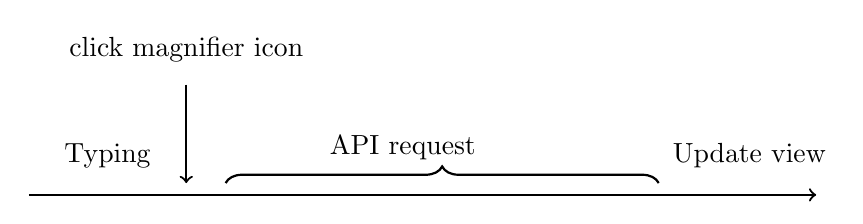
\begin{tikzpicture}[scale=1]
\node[align=center] at (1,0.5) {Typing};
\node[align=center] at (2,1.85) {click magnifier icon};
\draw [thick,->] (2,1.4) -- (2,0.15);
%\node[align=center] at (3.15,0.85) {Connect\\GPS};
%\draw [thick,decorate,decoration={brace,amplitude=6pt,raise=0pt}] (2.5,0.15) -- (3.75,0.15);
%\draw [thick,->] (4,0.85) -- (4,0.15);
\node[align=center] at (4.75,0.6) {API request};
%\draw [thick,->] (8.25,0.85) -- (8.25,0.15);
\node[align=center] at (9.15,0.5) {Update view};
\draw [thick,decorate,decoration={brace,amplitude=6pt,raise=0pt}] (2.5,0.15) -- (8,0.15);
\draw [thick,->] (0,0) -- (10,0);
%\draw [thick,->] (4.6,-0.85) -- (4.6,-0.15);
%\draw [thick,->] (7.65,-0.4) -- (7.65,-0.15);
%\draw [thick,decorate,decoration={brace,amplitude=6pt,raise=0pt,mirror}] (4.75,-0.15) -- (7.5,-0.15);
%\node[align=center] at (6.25,-0.85) {Symptomatic\\period};
%\node[align=center] at (4.6,-1.3) {Onset of\\symptoms};
\end{tikzpicture}
	\end{figure}

\end{frame}
\begin{frame}[fragile]
	\begin{figure}
		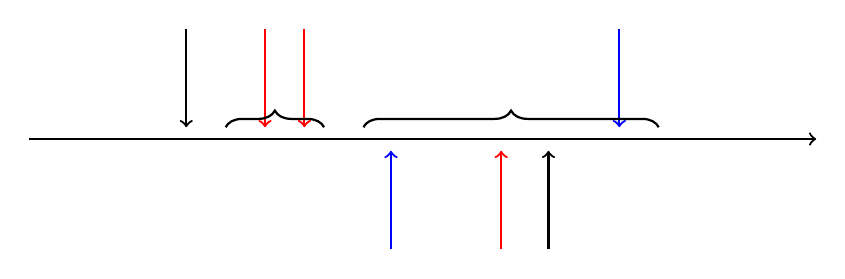
\begin{tikzpicture}[scale=1]
%\node[align=center] at (1,0.5) {Enter};
\draw [thick,->] (2,1.4) -- (2,0.15);
\draw [red, thick,->] (3,1.4) -- (3,0.15);
\draw [red, thick,->] (3.5,1.4) -- (3.5,0.15);
\draw [blue, thick,->] (7.5,1.4) -- (7.5,0.15);
\draw [blue, thick,->] (4.6,-1.4) -- (4.6,-0.15);
\draw [red, thick,->] (6.0,-1.4) -- (6.0,-0.15);
\draw [thick,->] (6.6,-1.4) -- (6.6,-0.15);
%\node[align=center] at (3.15,0.85) {Connect\\GPS};
\draw [thick,decorate,decoration={brace,amplitude=6pt,raise=0pt}] (2.5,0.15) -- (3.75,0.15);
%\draw [thick,->] (4,0.85) -- (4,0.15);
%\node[align=center] at (6.25,0.6) {API request};
%\draw [thick,->] (8.25,0.85) -- (8.25,0.15);
%\node[align=center] at (9.15,0.5) {Update view};
\draw [thick,decorate,decoration={brace,amplitude=6pt,raise=0pt}] (4.25,0.15) -- (8,0.15);
\draw [thick,->] (0,0) -- (10,0);
%\draw [thick,->] (4.6,-0.85) -- (4.6,-0.15);
%\draw [thick,->] (7.65,-0.4) -- (7.65,-0.15);
%\draw [thick,decorate,decoration={brace,amplitude=6pt,raise=0pt,mirror}] (4.75,-0.15) -- (7.5,-0.15);
%\node[align=center] at (6.25,-0.85) {Symptomatic\\period};
%\node[align=center] at (4.6,-1.3) {Onset of\\symptoms};
\end{tikzpicture}
	\end{figure}
\end{frame}



\begin{frame}[fragile]
\begin{columns}
\begin{column}{0.5\textwidth}
	\begin{center}
	\begin{figure}
		\centering
		
\includegraphics[height=.6\textheight]{tip}
	\end{figure}
	\end{center}
\end{column}
\begin{column}{0.6\textwidth}
	\begin{itemize}
		\item Delays
		\item User inputs 
		\item Failures (connectivity, gps on mobile devices)
		\item Sort api responses by time
		\item \emph{android/ios lifecycle}, etc
	\end{itemize}
\end{column}
\end{columns}

\end{frame}

\begin{frame}[fragile]
	\begin{figure}
		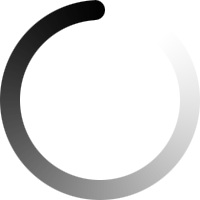
\includegraphics[width=.6\textwidth]{loading}
	\end{figure}
\end{frame}
\begin{frame}[fragile]
	Naive approach: put constrains in place to restrict the combinatorial range of possible options  
	\begin{itemize}
		\item Conditionally forbid user events (disable buttons, loading spinners, etc) 
		\item Boolean flags 
		\item Be defensive (if/else) 
		\item Bind/unbind from lifecycle , etc
	\end{itemize}
	(Or more technical constrains like single thread executors, queues, synchronization, etc)
\end{frame}

\begin{frame}
	The approach 
	\begin{itemize}
		\item doesn't scale. 
	\begin{itemize}
		\item pre-fatching
		\item background upload
		\item recovery/retry logic 
		\item debouncing, timeouts 
		\item no control on platform lifecycle
	\end{itemize}
\item can result in slower execution 
	\end{itemize}
	Slows down the performance/experience, unlocking parallelism will make things worst 
\end{frame}
\begin{frame}[fragile]
	Key motivators:
	\begin{itemize}
		\item Scalability/performance (both server-side  and client-side) 
		\item Better user experience 
	\end{itemize}



\end{frame}

\begin{frame}[fragile]
	``Concurrency is the composition of independently executing processes, typically functions, but they don't have to be.''

	``Parallelism is the simultaneous execution of multiple things, possibly related, possibly not.''

Rob Pike

\end{frame}
\begin{frame}[fragile]
	\begin{figure}
		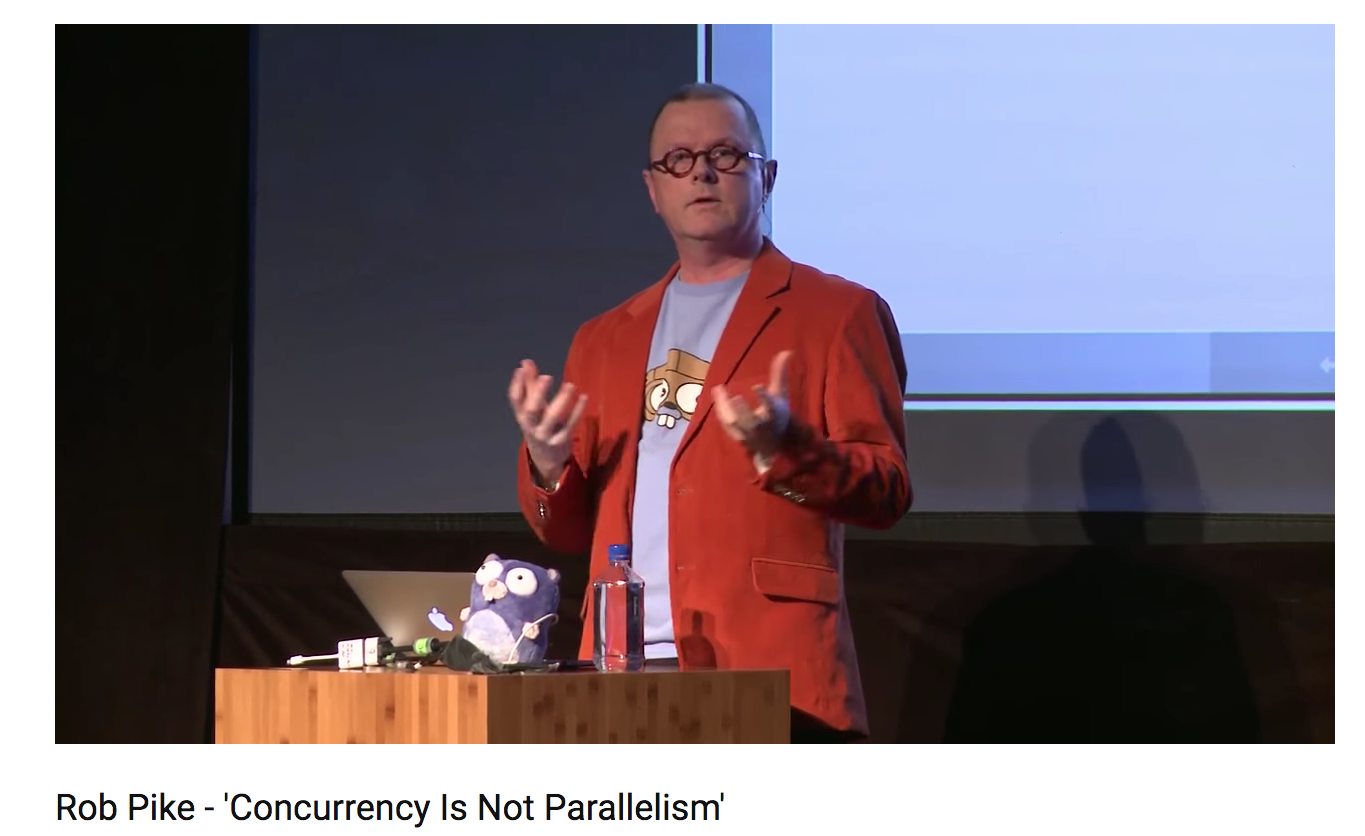
\includegraphics[height=.8\textheight]{rob_talk}
		\caption{\url{https://www.youtube.com/watch?v=cN_DpYBzKso&t=1061s}}
	\end{figure}
\end{frame}

\begin{frame}[fragile]
	\begin{figure}
		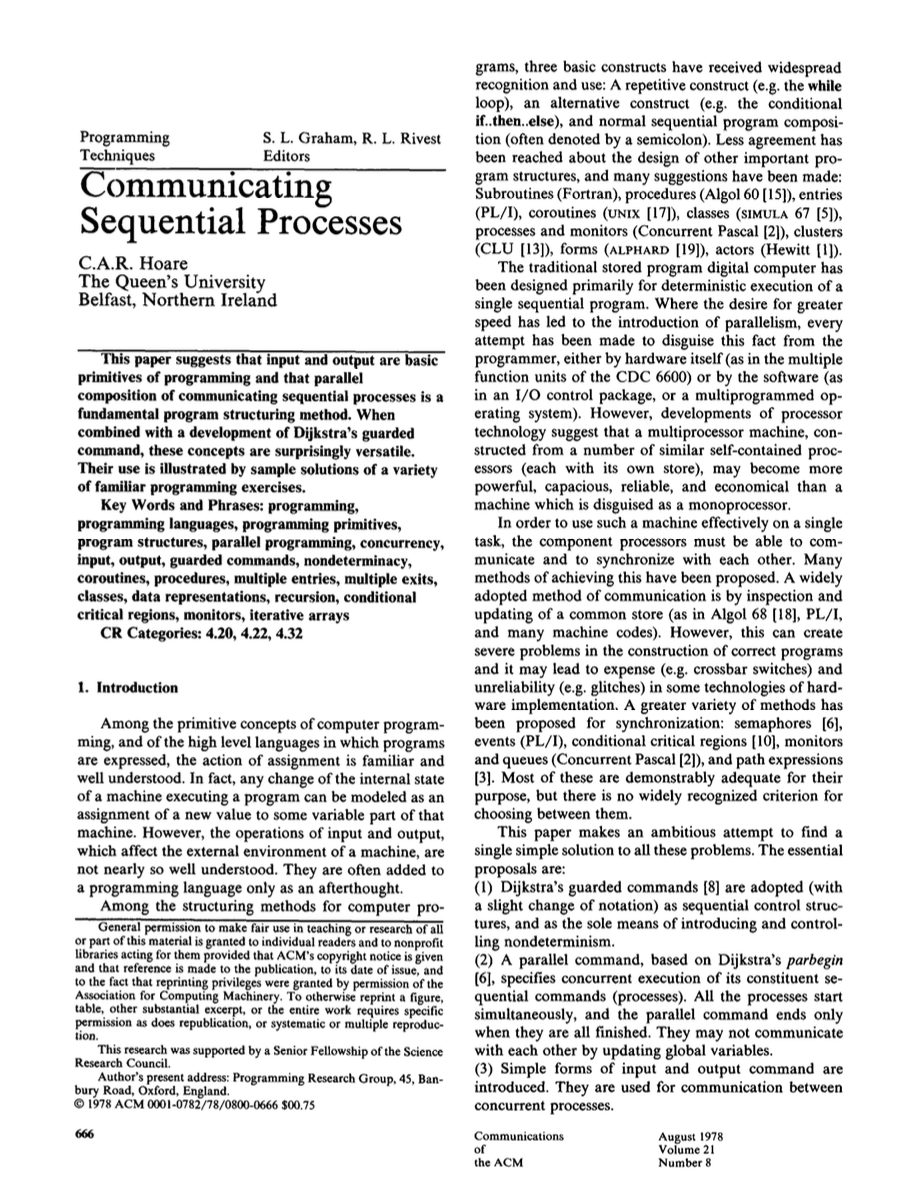
\includegraphics[height=.8\textheight]{tony}
		\caption{Tony Hoare's seminal paper}
	\end{figure}
\end{frame}
\begin{frame}[fragile]
``The most obvious application of the new ideas is to the specification, design,
and implementation of computer systems which continuously act and
interact with their environment. The basic idea is that these systems can be
readily decomposed into subsystems which operate concurrently and interact
with each other as well as with their common environment. The parallel composition
of subsystems is as simple as the sequential composition of lines or
statements in a conventional programming language.``

	Tony Hoare (CSP book, 2015)
\end{frame}



\begin{frame}[fragile]
	\begin{alertblock}{Concurrency}
		Two operations are concurrent if they are not ordered by \emph{happens before} relation%
		\footnote{Leslie Lamport's paper \url{https://www.microsoft.com/en-us/research/uploads/prod/2016/12/Time-Clocks-and-the-Ordering-of-Events-in-a-Distributed-System.pdf}}.
	\end{alertblock}
	

\end{frame}
\section{Blocking vs non-blocking}
\begin{frame}[fragile]
\begin{lstlisting}[language=Kotlin, basicstyle=\ttfamily]

/** inject resource here */

fun onClick() {
  val position = gpsService.getPositionFromGps()
  val locations = apiService.getLocations(position)
  view.showLocations(locations)
}
\end{lstlisting}
\end{frame}
\begin{frame}[fragile]
\begin{lstlisting}[language=Kotlin, basicstyle=\ttfamily]
typealias LatLng = Pair<Double, Double>

interface GpsService { 
    fun getPositionFromGps() : LatLng
}

interface ApiService { 
    fun getLocations(position : LatLng) 
             : List<String>
}
\end{lstlisting}
\end{frame}


%% LINE 
\mycomment{
\begin{frame}[fragile]
\begin{lstlisting}[language=Kotlin, basicstyle=\ttfamily]
fun onClick(){ 
   val coordinates = /*... put logic here */
   val data = /*... put http client here */
   view.showResults(data) 
}
\end{lstlisting}
\end{frame}
\begin{frame}[fragile]
	\begin{figure}
		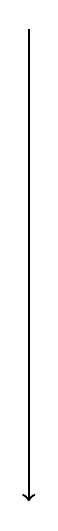
\begin{tikzpicture}[scale=1]
\draw [thick,->] (1,6) -- (1,0);
\end{tikzpicture}
	\end{figure}
\end{frame}
}
%% END LINE 

\begin{frame}[fragile]
\begin{lstlisting}[language=Kotlin, basicstyle=\ttfamily]
fun getLocations(position : LatLng) 
	     : List<String> {
		     
  /** Network request */
  Thread.sleep(3000)

  return listOf("etc")
}
\end{lstlisting}
\end{frame}
\begin{frame}[fragile]
	\begin{figure}
		\begin{tikzpicture}[scale=1]
			\node[align=left] at (1,6.5) {onClick()};
\draw [thick,->] (1,6) -- (1,4);
\draw [thick,->] (1,4) -- (4,4);
			\node[align=right] at (4,4.5) {getLocations()};
\draw [thick,->] (4,4) -- (4,2);
			\node[align=right] at (2.25,1.5) {return};
\draw [thick,->] (4,2) -- (1,2);
\draw [thick,->] (1,2) -- (1,0);
\end{tikzpicture}
	\end{figure}
\end{frame}
\begin{frame}[fragile]
\begin{lstlisting}[language=Kotlin, basicstyle=\ttfamily]
fun getLocations(position : LatLng) 
	     : List<String> {
		     
  val data = networkCall()
  return listOf(data)
}
\end{lstlisting}
\end{frame}
\begin{frame}[fragile]
	\begin{figure}
		\begin{tikzpicture}[scale=0.5]
\draw [thick,->] (1,6) -- (1,4);
\draw [thick,->] (1,4) -- (4,4);
\draw [thick,->] (4,4) -- (4,2);
\draw [thick,->] (4,2) -- (6,2);
\draw [thick,->] (6,2) -- (6,0);
\draw [thick,->] (6,0) -- (4,0);
\draw [thick,->] (4,0) -- (4,-2);
\draw [thick,->] (4,-2) -- (1,-2);
\draw [thick,->] (1,-2) -- (1,-4);
\end{tikzpicture}
	\end{figure}
\end{frame}

\begin{frame}[fragile]
\begin{lstlisting}[language=Kotlin, basicstyle=\ttfamily]
interface ApiService {

    fun getLocations(position : LatLng,
            callback : Callback): Unit

    interface Callback {
        fun onSuccess(locations : List<String>)
        fun onError(throwable : Throwable)
    }

}
\end{lstlisting}
\end{frame}
\begin{frame}[fragile]
	Few preliminary troubles 
	\begin{itemize}
		\item Unnatural contract (the output is represented via input)
		\item Don't chain nicely (callback hell, pyramid of doom, hadouken, etc) 
		\item Error propagation, and \ldots  
	\end{itemize}

\end{frame}
\begin{frame}[fragile]
	\ldots so far they don't solve our problem 
\begin{lstlisting}[language=Kotlin, basicstyle=\ttfamily]
fun getLocations(position: LatLng, 
         callback: ApiService.Callback) : Unit {
   Thread.sleep(3000)
   callback.onSuccess(listOf("etc"))
   return
}
\end{lstlisting}
\end{frame}
\begin{frame}[fragile]
\begin{lstlisting}[language=Kotlin, basicstyle=\ttfamily]
@Inject 
lateinit var executor : Executor 

fun getLocations(position: LatLng, 
            callback: ApiService.Callback) : Unit {
   executor.execute {
       Thread.sleep(3000)
       callback.onSuccess(listOf("etc"))
   }
   return
}
\end{lstlisting}
\end{frame}
\begin{frame}[fragile]
	\begin{alertblock}{Question}
		How do callbacks work when the programming language is single-thread?
	\end{alertblock}
\end{frame}
\begin{frame}[fragile]
	Now the \emph{consumer} of the service is \emph{not} blocked (it does not have to wait until completion).

	However, 
	\begin{itemize}
		\item we have to update the view on the UI thread, 
		\item the thread running the runnable is blocked  $\rightarrow$ thread pools, etc
	\end{itemize}

\end{frame}


\begin{frame}[fragile]
	Another option: Futures 
\begin{lstlisting}[language=Kotlin, basicstyle=\ttfamily]
interface ApiService {

    fun getLocations(position : LatLng): 
      Future<List<String>>

}
\end{lstlisting}
	Monadic chainability, error handling, etc (not in this talk :) ) 
\end{frame}
\section{Kotlin coroutines demystified }
\begin{frame}
	\begin{figure}
		\centering
		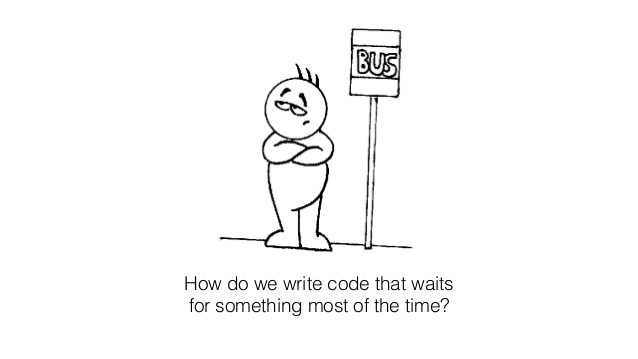
\includegraphics[width=.9\textwidth]{waiting}
	\end{figure}
\end{frame}
\begin{frame}[fragile]
\begin{lstlisting}[language=Kotlin, basicstyle=\ttfamily]
typealias LatLng = Pair<Double, Double>

interface GpsService { 
    suspend fun getPositionFromGps() : LatLng
}

interface ApiService { 
    suspend fun getLocations(position : LatLng) 
             : List<String>
}
\end{lstlisting}
\end{frame}

\begin{frame}
	Questions:
	\begin{itemize}
		\item How to implement the body of the suspend function? 
		\item How to invoke a suspend function?
	\end{itemize}
	
	This means respectively 
	\begin{itemize}
		\item How does the corotuine know when to pause/suspend?
		\item How does the coroutine know what to execute when the suspend function resumes?
	\end{itemize}
\end{frame}


% What happens to the caller 
% What happent to the body 

\begin{frame}[fragile]
%\begin{lstlisting}[language=Kotlin, basicstyle=\ttfamily]
%\end{lstlisting}
\end{frame}
\section{Coroutines-powered concurrency models}
\begin{frame}[fragile]
	Disadvantages of Java locking:
	\begin{itemize}
		\item Hard to maintain and error prone
		\item Priority inversion 
		\item Resumption can be expensive 
		\item Wasting resources 
	\end{itemize} 
\end{frame}
\begin{frame}[fragile]
\begin{itemize}
	\item CSP (aka, channels) 
\item actors 
	\end{itemize}
\end{frame}
\plain{Questions?}

%\begin{frame}[allowframebreaks] {References}
% \bibliography{demo}
% \bibliographystyle{abbrv}
%\end{frame}

\end{document}
\begin{lstlisting}[language=Kotlin, basicstyle=\ttfamily]
\end{lstlisting}

\begin{frame}
\begin{lstlisting}[language=Kotlin, basicstyle=\ttfamily]
\end{lstlisting}
\end{frame}
